\chapter{Quantum Electrodynamics and External States}
\label{ch:qed-external-states}

\section{Charged Spinors and Abelian Gauge Representatives}

The free theories constructed in the preceding chapters can be coupled by
letting a Dirac spinor field carry a one-dimensional unitary representation
of an Abelian gauge group. Let \(g\in\R\) be the charge of the spinor field.
For the electron convention used below,
\[
  g=-e,\qquad e>0 .
\]
The representative fields are
\[
  A_\mu(x),\qquad \psi_\alpha(x),\qquad \bar\psi^\alpha(x),
\]
where \(A_\mu\) is a real vector-potential representative and
\(\bar\psi=\psi^\dagger\beta\) is the Dirac adjoint defined in
Chapter~\ref{ch:spinor-fields-fermionic-path-integrals}.
A real function \(\xi(x)\) changes representatives by
\[
  A_\mu\mapsto A_\mu+\partial_\mu\xi,\qquad
  \psi\mapsto \ee^{\ii g\xi}\psi,\qquad
  \bar\psi\mapsto \bar\psi\,\ee^{-\ii g\xi}.
\]
The Abelian covariant derivative is
\[
  D_\mu\psi
  =
  \partial_\mu\psi-\ii gA_\mu\psi .
\]
It transforms with the same charge as \(\psi\):
\[
\begin{aligned}
  D_\mu(\ee^{\ii g\xi}\psi)
  &=
  \partial_\mu(\ee^{\ii g\xi}\psi)
  -\ii g(A_\mu+\partial_\mu\xi)\ee^{\ii g\xi}\psi  \\
  &=
  \ee^{\ii g\xi}D_\mu\psi .
\end{aligned}
\]
Thus the local action
\[
  S_{\mathrm{QED}}[A,\bar\psi,\psi]
  =
  \int\dd^4x\,
  \left[
    -\frac14F_{\mu\nu}F^{\mu\nu}
    -\bar\psi(\gamma^\mu D_\mu+m)\psi
  \right]
\]
is invariant under the representative change. Here
\[
  F_{\mu\nu}=\partial_\mu A_\nu-\partial_\nu A_\mu,\qquad
  \not a=a_\mu\gamma^\mu
\]
for any covector \(a_\mu\). Expanding the covariant derivative gives
\[
  \mathcal L_{\mathrm{QED}}
  =
  -\frac14F_{\mu\nu}F^{\mu\nu}
  -\bar\psi(\not\partial+m)\psi
  +\ii gA_\mu\bar\psi\gamma^\mu\psi .
\]
The last term is the interaction. In these gamma-matrix conventions the
electric current represented by the coupling to \(A_\mu\) is
\[
  j^\mu=\ii g\,\bar\psi\gamma^\mu\psi .
\]
It is invariant under the local Abelian representative change.

\section{Local Observables and Charged Insertions}

A local observable is represented by a local expression in the fields that is
invariant under all compactly supported changes of gauge representative.
Examples are
\[
  F_{\mu\nu},\qquad
  \bar\psi\psi,\qquad
  \ii g\,\bar\psi\gamma^\mu\psi .
\]
A local monomial containing \(N_\psi\) factors of \(\psi\) and
\(N_{\bar\psi}\) factors of \(\bar\psi\) has local charge
\[
  g(N_\psi-N_{\bar\psi}) .
\]
Gauge invariance of a pointlike local monomial therefore requires the net
local charge to vanish.

Charged insertions are represented by adding dressing data. Let \(C_x\) be an
oriented curve beginning at \(x\) and ending at a prescribed asymptotic
endpoint. For gauge parameters that vanish at that endpoint, define
\[
  \Psi_{C_x}(x)
  =
  \exp\left(\ii g\int_{C_x} A_\mu(y)\,\dd y^\mu\right)\psi(x).
\]
Indeed,
\[
  \int_{C_x}\partial_\mu\xi(y)\,\dd y^\mu
  =
  \xi(\infty)-\xi(x)
  =
  -\xi(x),
\]
so the phase acquired by the line integral cancels the phase of \(\psi(x)\).
The curve is part of the insertion: it records electromagnetic dressing data.
It is therefore not an additional pointlike local observable.

Similarly, for a path \(C_{y\to x}\) from \(y\) to \(x\),
\[
  \psi_\alpha(x)
  \exp\left(
    -\ii g\int_{C_{y\to x}} A_\mu(z)\,\dd z^\mu
  \right)
  \bar\psi^\beta(y)
\]
is invariant under compactly supported representative changes, because the
Wilson-line phase changes by
\[
  \exp\{-\ii g(\xi(x)-\xi(y))\}.
\]
This cancels the endpoint phases of \(\psi_\alpha(x)\) and
\(\bar\psi^\beta(y)\). The line operator itself may require short-distance
renormalization when it is defined as an operator-valued distribution. That
renormalization question is separate from the elementary gauge-covariance
calculation displayed here.

\begin{remark}
Gauge-fixed perturbation theory uses \(A_\mu,\psi,\bar\psi\) Green functions
as representative correlators. After gauge fixing these correlators have
propagators and vertices. Gauge-invariant local observables and physical
external photon states are read from \(F_{\mu\nu}\), helicity representatives,
and LSZ pole data.
\end{remark}

\section{Gauge-Fixed Generating Functional}

For perturbation theory choose the covariant gauge parameter
\(\xi_{\mathrm g}\) and add
\[
  \Delta\mathcal L
  =
  -\frac{1}{2\xi_{\mathrm g}}(\partial_\mu A^\mu)^2 .
\]
The Abelian Faddeev--Popov determinant for the condition
\(\partial_\mu A^\mu=\varphi\) is \(\det\Box\), independent of \(A_\mu\);
it is absorbed into the normalization of the generating functional.

Introduce an ordinary source \(J^\mu\) for \(A_\mu\), and Grassmann sources
\(\eta_\alpha,\bar\eta^\alpha\) for \(\bar\psi^\alpha,\psi_\alpha\). The
regulated Lorentzian generating functional, written in continuum shorthand, is
\[
\begin{aligned}
  Z[J,\bar\eta,\eta]
  &=
  \int DA\,D\bar\psi\,D\psi\,
  \exp\Biggl\{
    \ii\int\dd^4x\,
    \bigl(\mathcal L_{\mathrm{QED}}+\Delta\mathcal L\bigr) \\
  &\hspace{7em}
    +\ii\int\dd^4x\,
    \bigl(J^\mu A_\mu+\bar\eta\psi+\bar\psi\eta\bigr)
  \Biggr\}.
\end{aligned}
\]
As in the preceding finite-dimensional Berezin discussion, this notation is
shorthand for a regulated Gaussian integral followed by perturbative
expansion of the interaction term
\[
  \ii gA_\mu\bar\psi\gamma^\mu\psi
\]
around the Gaussian Maxwell and Dirac functionals already constructed. The
covariant gauge parameter \(\xi_{\mathrm g}\) changes representative
correlators; the local gauge-invariant correlators obtained from neutral
operators and field strengths do not depend on this representative choice.

The elementary momentum-space rules are as follows. A directed fermion line
from \(\psi_\alpha\) to \(\bar\psi^\beta\) carries
\[
\begin{tikzpicture}[baseline=-0.6ex,scale=0.82]
  \draw[thick,-{Stealth[length=3pt]}] (0,0) -- (1.8,0);
  \node[above] at (0.9,0) {\scriptsize \(k\)};
  \node[below] at (0,0) {\scriptsize \(\psi_\alpha\)};
  \node[below] at (1.8,0) {\scriptsize \(\bar\psi^\beta\)};
\end{tikzpicture}
\quad
=
\frac{-\ii(-\ii\not k+m)_\alpha{}^\beta}
     {k^2+m^2-\ii\epsilon}.
\]
The photon representative propagator is
\[
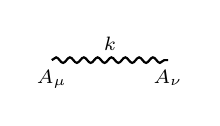
\begin{tikzpicture}[baseline=-0.6ex,scale=0.82]
  \draw[thick,decorate,decoration={snake,amplitude=1.0pt,segment length=5pt}]
    (0,0) -- (1.8,0);
  \node[above] at (0.9,0) {\scriptsize \(k\)};
  \node[below] at (0,0) {\scriptsize \(A_\mu\)};
  \node[below] at (1.8,0) {\scriptsize \(A_\nu\)};
\end{tikzpicture}
\quad
=
\frac{-\ii}{k^2-\ii\epsilon}
\left[
  \eta_{\mu\nu}
  -(1-\xi_{\mathrm g})\frac{k_\mu k_\nu}{k^2-\ii\epsilon}
\right].
\]
The cubic vertex with one photon representative and two spinor
representatives is
\[
\begin{tikzpicture}[baseline=-0.5ex,scale=0.82]
  \coordinate (v) at (0,0);
  \draw[thick,decorate,decoration={snake,amplitude=1.0pt,segment length=5pt}]
    (-1.0,0) -- (v);
  \draw[thick,-{Stealth[length=3pt]}] (v) -- (0.85,0.62);
  \draw[thick,-{Stealth[length=3pt]}] (0.85,-0.62) -- (v);
  \fill (v) circle (1.7pt);
  \node[left] at (-1.0,0) {\scriptsize \(\mu\)};
  \node[right] at (0.85,0.62) {\scriptsize \(\beta\)};
  \node[right] at (0.85,-0.62) {\scriptsize \(\alpha\)};
\end{tikzpicture}
\quad
=
-g(\gamma^\mu)_\beta{}^\alpha .
\]
For the electron convention \(g=-e\), the vertex factor is
\(e(\gamma^\mu)_\beta{}^\alpha\). The gauge parameter
\(\xi_{\mathrm g}\) appears only in the representative photon propagator.
Amplitudes between physical photon helicity states are obtained after LSZ
projection and are independent of the longitudinal representative.

\section{External Factors as Pole Data}

External factors in a diagrammatic amplitude are residues of poles already
identified by LSZ. The particle definitions have already been supplied by the
one-particle spectral data and scattering construction. With the normalizations
of Chapters 13, 16, and 18, the factors are
\[
\begin{array}{c|c}
\text{external state} & \text{LSZ factor} \\ \hline
e^-_{\mathrm{out}}(\vec p,\sigma)
&
\displaystyle
\frac{Z_\psi^{1/2}}{(2\pi)^{3/2}}\,
(\bar u^\sigma)^\alpha(\vec p)
\\[1.1em]
e^+_{\mathrm{out}}(\vec p,\sigma)
&
\displaystyle
\frac{Z_\psi^{1/2}}{(2\pi)^{3/2}}\,
v^\sigma_\alpha(\vec p)
\\[1.1em]
\gamma_{\mathrm{out}}(\vec k,h)
&
\displaystyle
\frac{Z_A^{1/2}}{(2\pi)^{3/2}\sqrt{2|\vec k|}}\,
e_\mu^{h*}(\vec k)
\\[1.1em]
e^-_{\mathrm{in}}(\vec p,\sigma)
&
\displaystyle
\frac{Z_\psi^{1/2}}{(2\pi)^{3/2}}\,
u^\sigma_\alpha(\vec p)
\\[1.1em]
e^+_{\mathrm{in}}(\vec p,\sigma)
&
\displaystyle
\frac{Z_\psi^{1/2}}{(2\pi)^{3/2}}\,
(\bar v^\sigma)^\alpha(\vec p)
\\[1.1em]
\gamma_{\mathrm{in}}(\vec k,h)
&
\displaystyle
\frac{Z_A^{1/2}}{(2\pi)^{3/2}\sqrt{2|\vec k|}}\,
e_\mu^h(\vec k).
\end{array}
\]
The free spinor or photon line adjacent to the external leg is not retained:
the LSZ operator removes that propagator and evaluates the residue at the
one-particle pole. The displayed spinor index is contracted with the
corresponding open index of the amputated Green-function kernel. In a
Fourier convention in which all momenta flow into a Green function, outgoing
massive particles are represented by the boundary value with the opposite
energy sign; the table above is written directly in terms of the physical
future-directed external momenta.

The massive spinor momenta satisfy
\[
  p^0=\omega_{\vec p}=\sqrt{\vec p^{\,2}+m^2},
\]
and the photon momentum satisfies
\[
  k^0=|\vec k|,\qquad k^2=0 .
\]
The spinors obey
\[
  (\not p-\ii m)u^\sigma(\vec p)=0,\qquad
  (\not p+\ii m)v^\sigma(\vec p)=0,
\]
with the corresponding adjoint equations for \(\bar u,\bar v\). The photon
polarization representatives obey
\[
  k^\mu e_\mu^h(\vec k)=0,\qquad
  e_\mu^h(\vec k)\sim e_\mu^h(\vec k)+\alpha k_\mu .
\]
For any polarization representative,
\[
  \not e^{\,h}(\vec k)=e_\mu^h(\vec k)\gamma^\mu .
\]

\begin{center}
\begin{tikzpicture}[>=Stealth,x=1cm,y=1cm]
  \tikzset{
    flowbox/.style={
      draw,
      rounded corners=2pt,
      align=center,
      font=\scriptsize,
      minimum height=0.72cm,
      text width=2.25cm
    },
    flowlabel/.style={font=\scriptsize,fill=white,inner sep=1.2pt}
  }
  \node[flowbox] (green) at (0,0) {gauge-fixed\\Green functions};
  \node[flowbox] (poles) at (3.35,0) {one-particle\\poles};
  \node[flowbox] (hard) at (6.7,0) {hard\\amplitude};
  \draw[->,thick] (green) -- node[flowlabel,above] {LSZ} (poles);
  \draw[->,thick] (poles) -- node[flowlabel,above] {residues} (hard);
  \draw[red!70!black,thick] (8.25,-0.72) -- (8.25,0.72);
  \node[red!70!black,align=center] at (9.35,0)
    {\scriptsize infrared\\[-0.1em]\scriptsize completion};
\end{tikzpicture}
\end{center}

The vertical mark in the diagram indicates a boundary of this chapter. The
hard-amplitude rules are perturbative rules for fixed external momenta and
helicities. The infrared completion of charged scattering is a further
construction.

Diagrammatically, the external factors attach to amputated kernels as follows:
\[
\begin{array}{cc}
\begin{tikzpicture}[baseline=(current bounding box.center),>=Stealth,scale=0.86]
  \tikzset{
    fermion/.style={line width=0.55pt,-{Stealth[length=3pt]}},
    blob/.style={circle,draw,fill=gray!16,minimum size=0.72cm,inner sep=0pt}
  }
  \node[blob] (b) at (1.25,0) {};
  \draw[fermion] (0,0)--(b);
  \node[below] at (0.62,-0.05) {\scriptsize \(u_\alpha^\sigma(\vec p)\)};
\end{tikzpicture}
&
\begin{tikzpicture}[baseline=(current bounding box.center),>=Stealth,scale=0.86]
  \tikzset{
    fermion/.style={line width=0.55pt,-{Stealth[length=3pt]}},
    blob/.style={circle,draw,fill=gray!16,minimum size=0.72cm,inner sep=0pt}
  }
  \node[blob] (b) at (0,0) {};
  \draw[fermion] (b)--(1.25,0);
  \node[below] at (0.85,-0.05) {\scriptsize \((\bar u^\sigma)^\alpha(\vec p)\)};
\end{tikzpicture}
\\[1.5em]
\begin{tikzpicture}[baseline=(current bounding box.center),>=Stealth,scale=0.86]
  \tikzset{
    photon/.style={decorate,decoration={snake,amplitude=1.1pt,segment length=5pt},line width=0.55pt},
    blob/.style={circle,draw,fill=gray!16,minimum size=0.72cm,inner sep=0pt}
  }
  \node[blob] (b) at (1.25,0) {};
  \draw[photon] (0,0)--(b);
  \node[below] at (0.55,-0.05) {\scriptsize \(e_\mu^h(\vec k)\)};
\end{tikzpicture}
&
\begin{tikzpicture}[baseline=(current bounding box.center),>=Stealth,scale=0.86]
  \tikzset{
    photon/.style={decorate,decoration={snake,amplitude=1.1pt,segment length=5pt},line width=0.55pt},
    blob/.style={circle,draw,fill=gray!16,minimum size=0.72cm,inner sep=0pt}
  }
  \node[blob] (b) at (0,0) {};
  \draw[photon] (b)--(1.25,0);
  \node[below] at (0.82,-0.05) {\scriptsize \(e_\mu^{h*}(\vec k)\)};
\end{tikzpicture}
\end{array}
\]
with the common normalization factors displayed in the table.

\section{Compton Scattering at Tree Level}

Consider the process
\[
  e^-(p,\sigma)+\gamma(k,h)
  \longrightarrow
  e^-(p',\sigma')+\gamma(k',h')
\]
with
\[
  p+k=p'+k' .
\]
At tree level two diagrams contribute:
\[
\begin{tikzpicture}[scale=0.93,baseline=(current bounding box.center)]
  \tikzset{
    photon/.style={decorate,decoration={snake,amplitude=1.1pt,segment length=5pt},line width=0.58pt}
  }
  \begin{scope}
    \draw[thick,-{Stealth[length=3pt]}] (0,0) -- (1.25,0) -- (2.5,0);
    \draw[photon,-{Stealth[length=3pt]}] (0.55,1.0) -- (0.98,0.08);
    \draw[photon,-{Stealth[length=3pt]}] (1.52,0.08) -- (1.95,1.0);
    \node[below] at (0,0) {\scriptsize \(p\)};
    \node[below] at (1.25,0) {\scriptsize \(p+k\)};
    \node[below] at (2.5,0) {\scriptsize \(p'\)};
    \node[above] at (0.52,1.0) {\scriptsize \(k\)};
    \node[above] at (2.0,1.0) {\scriptsize \(k'\)};
  \end{scope}
  \node at (3.05,0.22) {\Large \(+\)};
  \begin{scope}[xshift=3.75cm]
    \draw[thick,-{Stealth[length=3pt]}] (0,0) -- (1.25,0) -- (2.5,0);
    \draw[photon,-{Stealth[length=3pt]}] (0.55,1.0) -- (0.98,0.08);
    \draw[photon,-{Stealth[length=3pt]}] (1.52,0.08) -- (1.95,1.0);
    \node[below] at (0,0) {\scriptsize \(p\)};
    \node[below] at (1.25,0) {\scriptsize \(p-k'\)};
    \node[below] at (2.5,0) {\scriptsize \(p'\)};
    \node[above] at (0.52,1.0) {\scriptsize \(k'\)};
    \node[above] at (2.0,1.0) {\scriptsize \(k\)};
  \end{scope}
\end{tikzpicture}
\]
After removing the factor
\[
  (2\pi)^4\delta^4(p+k-p'-k')
\]
from the scattering matrix element, the reduced amplitude is
\[
\begin{aligned}
  \ii\mathcal M
  &=
  \frac{-\ii e^2}
       {(2\pi)^6\sqrt{2|\vec k|}\sqrt{2|\vec k'|}}\,
  \bar u^{\sigma'}(\vec p')
  \Biggl[
    \not e^{\,h'*}(\vec k')\,
    \frac{-\ii(\not p+\not k)+m}
         {(p+k)^2+m^2-\ii\epsilon}\,
    \not e^{\,h}(\vec k)  \\
  &\hspace{8.7em}
    +
    \not e^{\,h}(\vec k)\,
    \frac{-\ii(\not p-\not k')+m}
         {(p-k')^2+m^2-\ii\epsilon}\,
    \not e^{\,h'*}(\vec k')
  \Biggr]
  u^\sigma(\vec p).
\end{aligned}
\]
This is an LSZ-reduced expression: the external spinors and polarization
vectors are the pole residues listed above.

The expression descends from photon representatives to photon helicity states.
Let
\[
  N(q)=-\ii\not q+m,\qquad D(q)=q^2+m^2-\ii\epsilon .
\]
If the incoming polarization is shifted by
\[
  e_\mu^h(k)\mapsto e_\mu^h(k)+\alpha k_\mu ,
\]
then the first diagram changes by a factor proportional to
\[
  \frac{N(p+k)\not k}{D(p+k)}u^\sigma(p).
\]
Using \(p^2=-m^2\), \(k^2=0\), and
\((\not p-\ii m)u^\sigma(p)=0\), one obtains
\[
  N(p+k)\not k\,u^\sigma(p)
  =
  -2\ii(p\cdot k)u^\sigma(p),
  \qquad
  D(p+k)=2p\cdot k-\ii\epsilon .
\]
Thus the first diagram contributes
\[
  -\ii\alpha\,
  \bar u^{\sigma'}(p')\not e^{\,h'*}(k')u^\sigma(p)
\]
up to the common prefactor. For the second diagram, momentum conservation
gives \(p-k'=p'-k\), and the adjoint Dirac equation gives
\[
  \bar u^{\sigma'}(p')\not k\,N(p-k')
  =
  -2\ii(p'\cdot k)\bar u^{\sigma'}(p'),
  \qquad
  D(p-k')=-2p'\cdot k-\ii\epsilon .
\]
The second diagram therefore contributes
\[
  +\ii\alpha\,
  \bar u^{\sigma'}(p')\not e^{\,h'*}(k')u^\sigma(p)
\]
with the same common prefactor. The two shifts cancel. The same argument
applies to shifts of the outgoing photon representative. This cancellation is
the tree-level Ward identity for the Compton amplitude.

With the cross-section normalization of
Chapter~\ref{ch:cross-sections-unitarity}, the total cross section
for fixed incoming spin and helicity is
\[
\begin{aligned}
  \sigma
  &=
  \frac{(2\pi)^6}{v}
  \int\dd^3\vec k'\,\dd^3\vec p'\,
  (2\pi)^4\delta^4(k+p-k'-p')  \\
  &\qquad\times
  \sum_{\substack{h'=\pm1\\ \sigma'=1,2}}
  \left|
    \mathcal M(\vec p',\sigma';\vec k',h'
    \mid
    \vec p,\sigma;\vec k,h)
  \right|^2 ,
\end{aligned}
\]
where \(v\) is the incoming relative velocity. The evaluation of the spin
and polarization sums is a kinematic exercise built from the completeness
relations of Chapters 16 and 17.

\section{Infrared Boundary of Charged Scattering}

The perturbative rules above are rules for hard Green-function residues. They
are valid order by order once an infrared regulator or an inclusive
prescription has been specified. The exact long-range theory has an additional
structural feature: Gauss' law ties electric charge to an electromagnetic
field extending to arbitrarily large distances. Consequently the charged-sector
asymptotic data is infrared-sensitive: its spectral support is tied to the
charged mass threshold together with arbitrarily soft radiation. This lies
outside the isolated massive-particle hypothesis used in the basic
Haag--Ruelle construction.

This boundary is already visible in the charged dressing
\(\Psi_{C_x}(x)\). A dressing that retains nonzero electric charge extends to
infinity. In scattering, the same long-range field is represented
perturbatively by arbitrarily soft photons.
The physical completions are inclusive transition probabilities, where soft
photons below a resolution threshold are summed over, or dressed asymptotic
charged states. Those constructions belong after renormalization and the
analysis of infrared singularities. The present chapter supplies the
gauge-fixed hard-amplitude rules on which that later analysis acts.
